\documentclass{assignment}
\usepackage{enumitem}
\usepackage{graphicx}

\begin{document}
\assignmentTitle{Pham Xuan Hoang}{2640009}{assets/usth_logo.png}%
{Information Systems}{Labwork 4}

\begin{figure}[h]
    \centering
    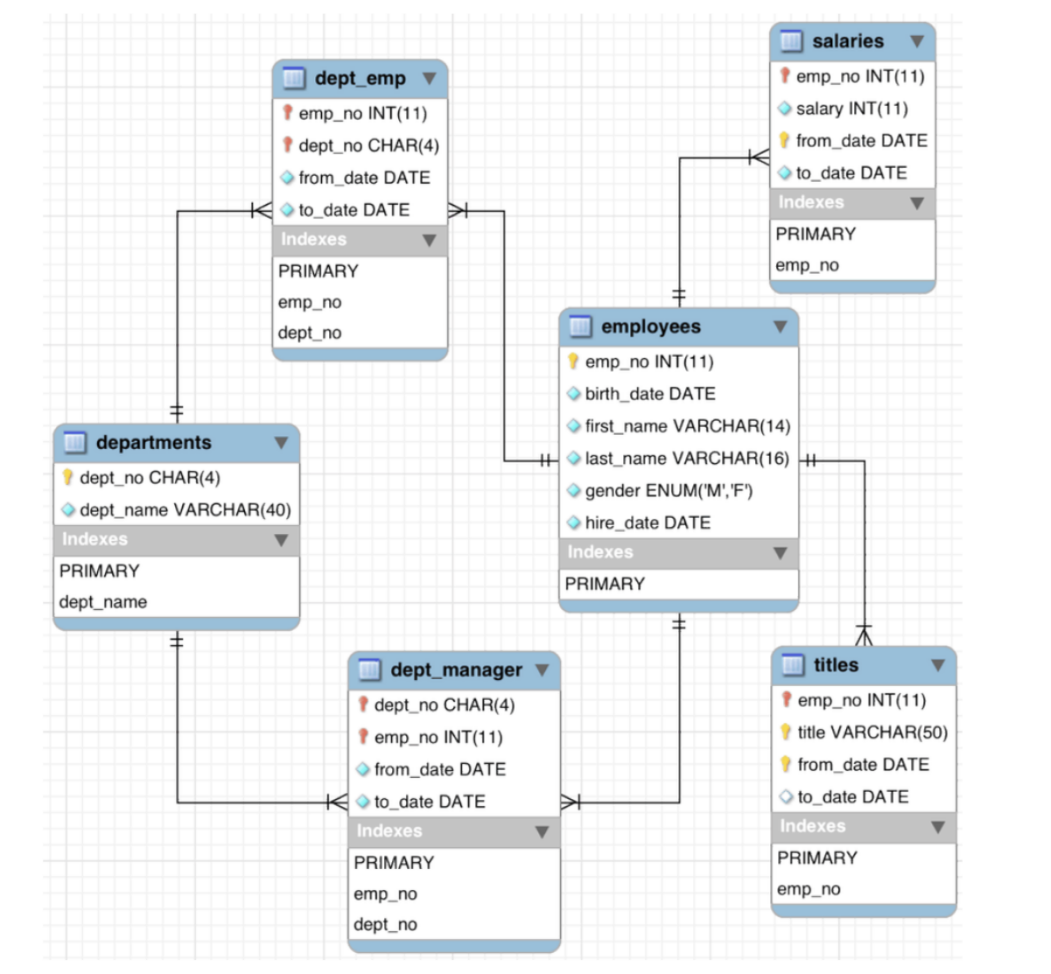
\includegraphics[width=0.7\linewidth]{assets/employees_schema.png}
    \caption{\texttt{employees} database schema}
\end{figure}

\section*{Built-in function}
Write SQL commands for the following queries:
\begin{itemize}[noitemsep]
    \item What is the average salary of each employee? (output shortened)
        \lstinputlisting[language=sql, firstline=4,
        lastline=9]{assets/complex_queries_a.sql}
        Output:
        \lstinputlisting[style=output, firstline=1,
        lastline=9]{assets/complex_queries_a_output.txt}
    \item How much was each employee paid in total? (output shortened)
        \lstinputlisting[language=sql, firstline=12,
        lastline=17]{assets/complex_queries_a.sql}
        Output:
        \lstinputlisting[style=output, firstline=10,
        lastline=18]{assets/complex_queries_a_output.txt}
    \item Minimum, maximum and total salaries of each department
        \lstinputlisting[language=sql, firstline=20,
        lastline=27]{assets/complex_queries_a.sql}
        Output:
        \lstinputlisting[style=output, firstline=19,
        lastline=31]{assets/complex_queries_a_output.txt}
    \item Which department paid more than 20 billion dollars for their employee
        \lstinputlisting[language=sql, firstline=30,
        lastline=37]{assets/complex_queries_a.sql}
        Output:
        \lstinputlisting[style=output, firstline=32,
        lastline=38]{assets/complex_queries_a_output.txt}
    \item Total salaries of male employees in each department
        \lstinputlisting[language=sql, firstline=40,
        lastline=48]{assets/complex_queries_a.sql}
        Output:
        \lstinputlisting[style=output, firstline=39,
        lastline=51]{assets/complex_queries_a_output.txt}
    \item Total salaries of department managers for each department,
        from highest to lowest
        \lstinputlisting[language=sql, firstline=51,
        lastline=58]{assets/complex_queries_a.sql}
        Output:
        \lstinputlisting[style=output, firstline=52,
        lastline=64]{assets/complex_queries_a_output.txt}
\end{itemize}
\section*{Subquery}
Write SQL command for the following queries:
\begin{itemize}[noitemsep]
    \item Who have the same name as the managers of the ``Finance'' department
        \lstinputlisting[language=sql, firstline=3,
        lastline=21]{assets/complex_queries_b.sql}
        Output:
        \lstinputlisting[style=output, firstline=1,
        lastline=1]{assets/complex_queries_b_output.txt}
    \item Who in the ``Production'' department were hired after the
        promotion of the last manager in that department
        \lstinputlisting[language=sql, firstline=24,
        lastline=38]{assets/complex_queries_b.sql}
        Output:
        \lstinputlisting[style=output, firstline=2,
        lastline=12]{assets/complex_queries_b_output.txt}
        \newpage
    \item Find the average salary of each department, from highest to lowest
        \lstinputlisting[language=sql, firstline=41,
        lastline=58]{assets/complex_queries_b.sql}
        Output:
        \lstinputlisting[style=output, firstline=13,
        lastline=25]{assets/complex_queries_b_output.txt}
    \item Find the average salary for each type of Engineer, from
        highest to lowest
        \lstinputlisting[language=sql, firstline=61,
        lastline=79]{assets/complex_queries_b.sql}
        \newpage
        Output:
        \lstinputlisting[style=output, firstline=26,
        lastline=32]{assets/complex_queries_b_output.txt}
\end{itemize}

\section*{View}
Write SQL command for the following queries:
\begin{itemize}[noitemsep]
    \item Who have the same name as the managers of the ``Finance'' department
        \lstinputlisting[language=sql, firstline=3,
        lastline=14]{assets/complex_queries_c.sql}
        Output:
        \lstinputlisting[style=output, firstline=1,
        lastline=1]{assets/complex_queries_c_output.txt}
    \item Who in the ``Production'' department were hired after the
        promotion of the last manager in that department
        \lstinputlisting[language=sql, firstline=24,
        lastline=40]{assets/complex_queries_c.sql}
        Output:
        \lstinputlisting[style=output, firstline=2,
        lastline=12]{assets/complex_queries_c_output.txt}
    \item Find the average salary of each department, from highest to lowest
        \lstinputlisting[language=sql, firstline=43,
        lastline=61]{assets/complex_queries_c.sql}
        Output:
        \lstinputlisting[style=output, firstline=13,
        lastline=25]{assets/complex_queries_c_output.txt}
    \item Find the average salary for each type of Engineer, from
        highest to lowest
        \lstinputlisting[language=sql, firstline=64,
        lastline=82]{assets/complex_queries_c.sql}
        \newpage
        Output:
        \lstinputlisting[style=output, firstline=26,
        lastline=32]{assets/complex_queries_c_output.txt}
\end{itemize}

\section*{Review}
\begin{figure}[h]
    \centering
    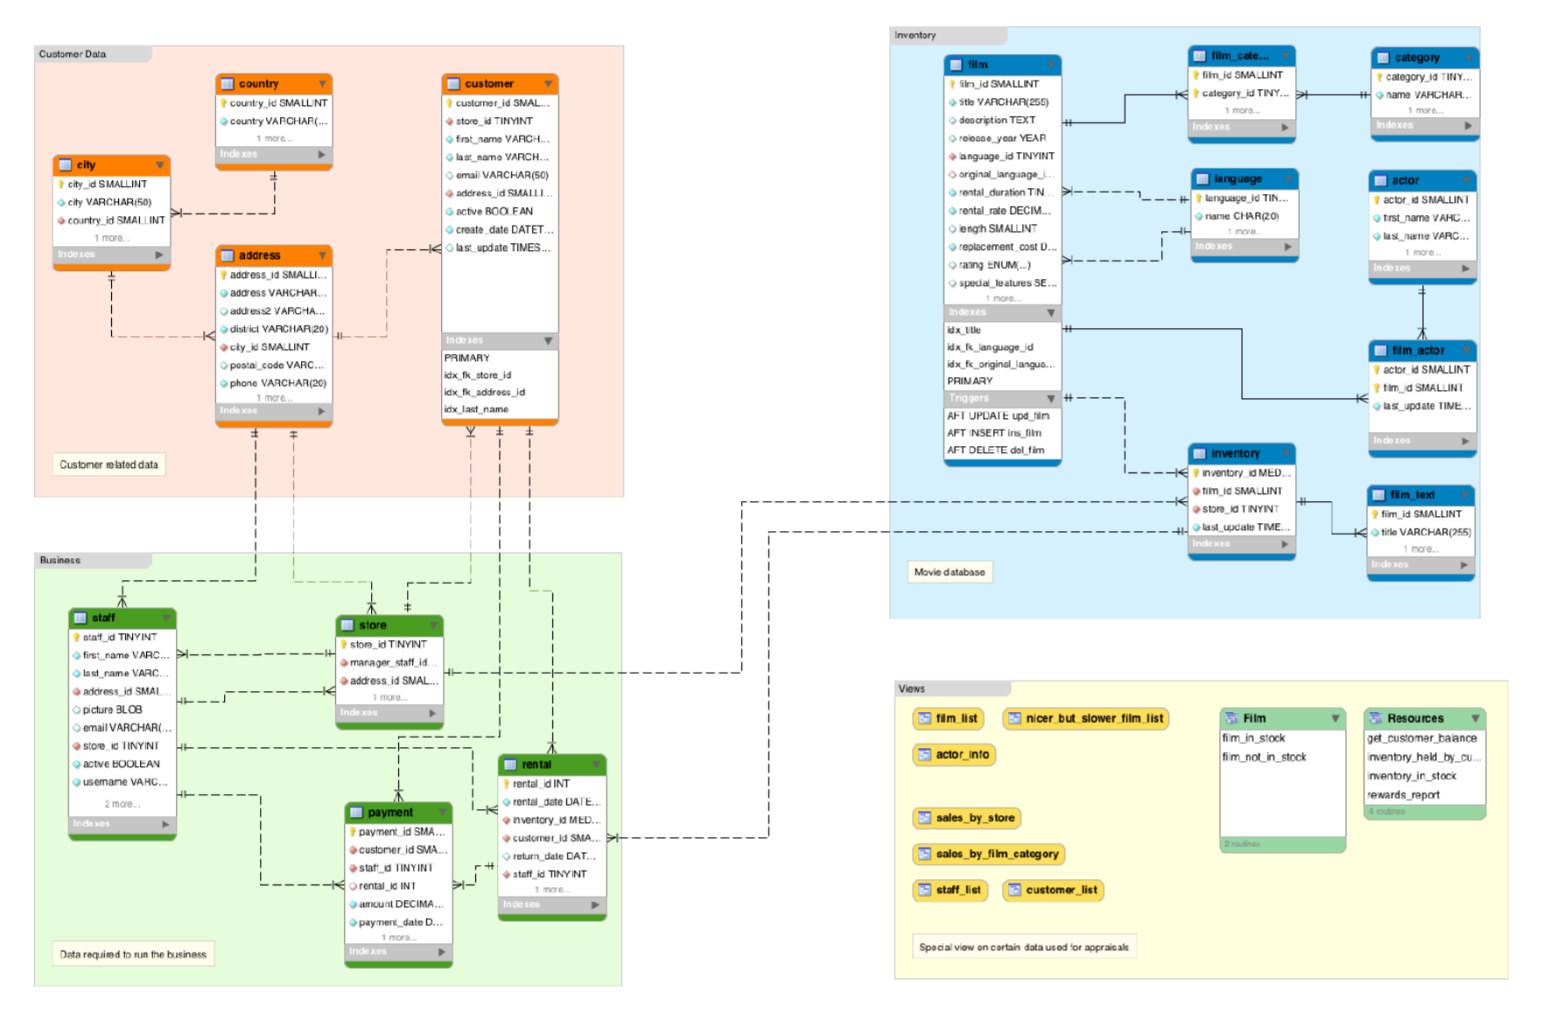
\includegraphics[width=0.7\linewidth]{assets/sakila_schema.png}
    \caption{\texttt{sakila} database schema}
\end{figure}

\begin{itemize}[noitemsep]
    \item List names of all the languages in the database (sorted
        alphabetically)
        \lstinputlisting[language=sql, firstline=3,
        lastline=5]{assets/review.sql}
        Output:
        \lstinputlisting[style=output, firstline=1,
        lastline=10]{assets/review_output.txt}
    \item List full names of actors with ``GER'' in their last name,
        ordered by their first name
        \lstinputlisting[language=sql, firstline=8,
        lastline=11]{assets/review.sql}
        \newpage
        Output:
        \lstinputlisting[style=output, firstline=11,
        lastline=20]{assets/review_output.txt}
    \item Find all the addresses where postal code starts with
        ``57'', and return addresses sorted.
        \lstinputlisting[language=sql, firstline=16,
        lastline=21]{assets/review.sql}
        Output:
        \lstinputlisting[style=output, firstline=21,
        lastline=35]{assets/review_output.txt}
    \item How many films involve a ``DWARF'' in their titles?
        \lstinputlisting[language=sql, firstline=24,
        lastline=24]{assets/review.sql}
        Output:
        \lstinputlisting[style=output, firstline=36,
        lastline=40]{assets/review_output.txt}
    \item Find full names of actors who played in a film involving
        ``WAR'' in title and longer than 2.5 hours, along with the
        title, run length and release year of the movie. Sorted by
        the actors last names. (output shortened)
        \lstinputlisting[language=sql, firstline=30,
        lastline=48]{assets/review.sql}
        Output:
        \lstinputlisting[style=output, firstline=41,
        lastline=47]{assets/review_output.txt}
    \item Find all the film categories in which there are between 55
        and 65 films. Return the names of these categories and the
        number of films per category, sorted by the number of films descending.
        \lstinputlisting[language=sql, firstline=53,
        lastline=60]{assets/review.sql}
        Output:
        \lstinputlisting[style=output, firstline=48,
        lastline=61]{assets/review_output.txt}
    \item In how many film categories is the average difference between
        the film replacement cost and the rental rate larger than 17?
        \lstinputlisting[language=sql, firstline=64,
        lastline=85]{assets/review.sql}
        Alternate approach using \texttt{CREATE VIEW}
        \lstinputlisting[language=sql, firstline=88,
        lastline=111]{assets/review.sql}
        Output:
        \lstinputlisting[style=output, firstline=62,
        lastline=73]{assets/review_output.txt}
    \item Find the address district(s) name(s) such that the minimal
        postal code in the district(s) is maximal over all the districts.
        Make sure your query ignores empty postal codes and district
        names.
        \lstinputlisting[language=sql, firstline=116,
        lastline=128]{assets/review.sql}
        Output:
        \lstinputlisting[style=output, firstline=86,
        lastline=90]{assets/review_output.txt}
    \item Find the names (first and last) of all the actors and customers
        whose first name is the same as the first name of the actor
        with ID 101 (exclude the actor with ID 101).
        \lstinputlisting[language=sql, firstline=133,
        lastline=150]{assets/review.sql}
        Output:
        \lstinputlisting[style=output, firstline=91,
        lastline=97]{assets/review_output.txt}
\end{itemize}
\end{document}
